%% ==============================
\chapter{\iflanguage{ngerman}{Ergebnisse}{Results}}
\label{sec:results}
%% ==============================
\section{Hardware and Setup for the Evaluation}\label{c6_sec_setup_all}
\subsection{Hardware}
The evaluation was conducted on real hardware. For the evaluation, multiple computers as well as multiple robots were used. In the following, a short overview of the computers and robots is given. The placement of the robots is described, and the different setups for the evaluation are explained.




\subsubsection{Computers}
\begin{wrapfigure}{r}{6cm}
\includegraphics[width=6cm]{Figures/c6/network_setup.pdf}
\caption{Schematic overview of the network setup.} \label{c6_fig_network}
\end{wrapfigure}
The used computers are three off the shelf laptops. They are not specially designed for control or real-time tasks. A detailed overview of the exact hardware specifications of the used laptops is shown in Table \ref{c3_tab_pc_overview}. 
It includes the processor and network card, as well as the size of the RAM and what type of RAM was used. The first computer (PC1) is a Tuxedo Polaris AMD Gen3. The second one (PC2) a Lenovo Legion 5 15ACH6H and the third computer (PC3) a Lenovo Legion 5 Pro 16ARH7H.\newline
The setup on the laptops itself was on each the same. A fresh Kubuntu 22.04 was installed. The real-time Kernel was installed via the Ubuntu "\texttt{pro}" command. Rolling was chosen as the \gls{ros2} distribution and the base of changes to the \gls{r2c} and the \textit{ros2\_controllers} repositories is listed in the \autoref{c3_tab_pc_overview}.
% Network card : lshw command
% cpu : lscpu
% memory: sudo dmidecode --type 17
% 1 -> arbeitslaptop
% 2 -> mein laptop
% 3 -> yaxin laptop



\subsubsection{Network}\label{c6_sec_network}
The network switch used in the experiments is a five port switch by NETGEAR. The model is called Prosafe Plus Switch (GS105Ev2). For the evaluation, the robots and computers were connected only over the switch in their own network, as shown in \autoref{c6_fig_network}. The computers were not connected to any other networks at the time the tests were conducted and except for the traffic created by the tests nothing else was routed over the network.



\subsubsection{Robots and Controller for the Evaluation}\label{c3_sec_used_robots}
The used robots for the evaluation are two industrial robots of the type KUKA KR 3 R540 \cite{noauthor_agile_nodate, noauthor_kuka_kr_3_agiluspdf_nodate}. One robot is depicted in \autoref{ca_fig_r2c_mr_is} on the left site. The robots are a 6-axis jointed-arm robots. They have a maximum reach of $541$ \si{\micro\meter} and a pose repeatability of about $\pm 0.002$ \si{\micro\meter}. The robots are embedded in the \textit{ready2\_educate} as shown in \autoref{c3_fig_r2c_mr_is} on the right site. On the flange is a pneumatic actuated Zimmer gp406 gripper mounted. The mount is probably specific designed for the \textit{ready2\_educate} platform, but unfortunately a CAD model for the mount could not be found. \newline
The joint naming convention is followed, meaning the joints are numbered in ascending alphanumeric order starting from the base (joint A1 or joint\_a1) to the flange joint (joint A6 or joint\_a6).\newline
The robot controller utilized in the platform is a KUKA KR C4 compact. The \acrfull{rsi}  was used for communication with the robot via the robot controller.
\begin{table}[htbp]
    \centering
\begin{tabular}{ |c|c|c|c| }
\hline
\multicolumn{4}{|c|}{Overview of PCs used for the evaluation} \\
\hline
& PC1 & PC2 & PC3  \\
\hline
\hline
\textbf{Hardware} &  &  & \\\hline
    Processor &
        \begin{minipage}{3.7cm}
	       \vskip 8pt
		      16 $\times$ AMD Ryzen 7 5800H with Radeon Graphics
	       \vskip 8pt
	    \end{minipage} & 
        \begin{minipage}{3.7cm}
    	    \vskip 8pt
    		   12 $\times$ AMD Ryzen 5 5600H with Radeon Graphics
    	    \vskip 8pt
	    \end{minipage} & 
        \begin{minipage}{3.7cm}
	       \vskip 8pt
		      16 $\times$ AMD Ryzen 7 6800H with Radeon Graphics
	       \vskip 8pt
	    \end{minipage} \\\hline
    RAM &
        \begin{minipage}{3.7cm}
	       \vskip 8pt
		      2 $\times$ 32GB DDR4 Samsung SODIMM 3200 MT/s
	       \vskip 8pt
	    \end{minipage} & 
        \begin{minipage}{3.7cm}
    	    \vskip 8pt
    		   2 $\times$ 16GB DDR4 SODIMM 3200 MT/s
    	    \vskip 8pt
	    \end{minipage} & 
        \begin{minipage}{3.7cm}
	       \vskip 8pt
		      2 $\times$ 16GB DDR5 SODIMM 4800 MT/s
	       \vskip 8pt
	    \end{minipage} \\\hline
    Network Card &
        \begin{minipage}{3.7cm}
	       \vskip 8pt
		      Realtek Semiconductor Co., LtdRTL8125 2.5GbE Controller 1Git/s
	       \vskip 8pt
	    \end{minipage} & 
        \begin{minipage}{3.7cm}
    	   \vskip 8pt
    		Realtek Semiconductor Co., RTL8111/ 8168/8411 PCI Express 1Gbit/s
    	   \vskip 8pt
	    \end{minipage} & 
        \begin{minipage}{3.7cm}
          \vskip 8pt
		      Realtek Semiconductor Co., RTL8111/ 8168/8411 PCI Express 1Gbit/s
	       \vskip 8pt
	    \end{minipage} \\\hline\hline
\textbf{Setup} & & & \\\hline
    Operating System & Kubuntu 22.04 &  Kubuntu 22.04 & Kubuntu 22.04 \\\hline
    Kernel & 5.15.0-1039-realtime & 5.15.0-1039-realtime & 5.15.0-1039-realtime  \\\hline
    Real-time Kernel & PREEMPT\_RT & PREEMPT\_RT & PREEMPT\_RT \\\hline
    ROS version & Rolling & Rolling & Rolling \\\hline
        \begin{minipage}{3cm}
        \vskip 4pt
    		   ros2\_control based on commit:\vskip 8pt
	    \end{minipage} & 0eb319ea43b78b886a & 0eb319ea43b78b886a & 0eb319ea43b78b886a \\\hline
            \begin{minipage}{3cm}
        \vskip 4pt
    		   ros2\_controllers based on commit:\vskip 8pt
	    \end{minipage} & 05d7a5ec73a02eab2c & 05d7a5ec73a02eab2c & 05d7a5ec73a02eab2c \\\hline
\end{tabular}
    \caption{Three different computers were used for the evaluation. The table gives an overview of the used hardware, as well as the setup on each of the computers.}
    \label{c3_tab_pc_overview}
\end{table}



\subsection{Description of the Test Setup}\label{c6_sec_description}
The fundamental idea for the evaluation was to couple the two robots at the TCP and then move the end effectors. The executed trajectories were chosen in such a way that the relative pose of the effectors TCPs to each other should stay the same during the
\begin{wrapfigure}{r}{8cm}
\includegraphics[width=8cm]{Figures/c6/schematic_messurement_rotation.pdf}
\caption{Mounting of the distance sensor on the gripper. 1A and 1B gripper housing of fist and second robot. 2 plate with an inclination. 3 the laser of the distance sensor. 4A and 4B exemplary rotation around aligned axes A6 of robots. 5 Aligned axes A6.} \label{c6_fig_schematic_gripper_mounting}
\end{wrapfigure}
 movement of the robots. \newline
 As performance metrics, the jitter and simultaneousness of the executed movement were measured from outside the system. This allowed for evaluation of the implemented concept regarding those performance metrics. Further, the impact of different \glspl{rmw} on the jitter and simultaneousness was investigated. \newline
 The coupling of was done with the distance sensor OD1-B035 Mini Pro from Sick. The sensor has a measuring range of $35\pm15$ \si{\milli\meter} and a resolution of $6$ \si{\micro\meter} with a repeatability of $9$ \si{\micro\meter}. As the measuring range of the distance sensor is very limited, the two \textit{ready2\_educate} platforms were placed front to front as shown in \autoref{c6_fig_robot_placement}. A start configuration, where the arm is fully extended to the front, was chosen. Then it was tried to align the axis of rotation of A6 as precise as possible. The distance sensor was then mounted as shown in \autoref{c6_fig_schematic_gripper_mounting}. The black rectangles with numbers 1A and 1B represent the housing of the gripper of the first and second robot. The gripper jaws are represented by the dark gray rectangles. One problem was that the grippers could not be disassembled from the flange. As a solution, a bracket for the distance sensor, which could be firmly gripped by the gripper, was created. This is represented by the dark blue rectangle. The distance sensor was then mounted on the bracket and the bracket fixed by the gripper. On the other gripper a plate, shown as number 2 in \autoref{c6_fig_schematic_gripper_mounting},  with an inclination was mounted. The distance change between the end effectors was measured.
\begin{figure}[htbp]
	\centering
	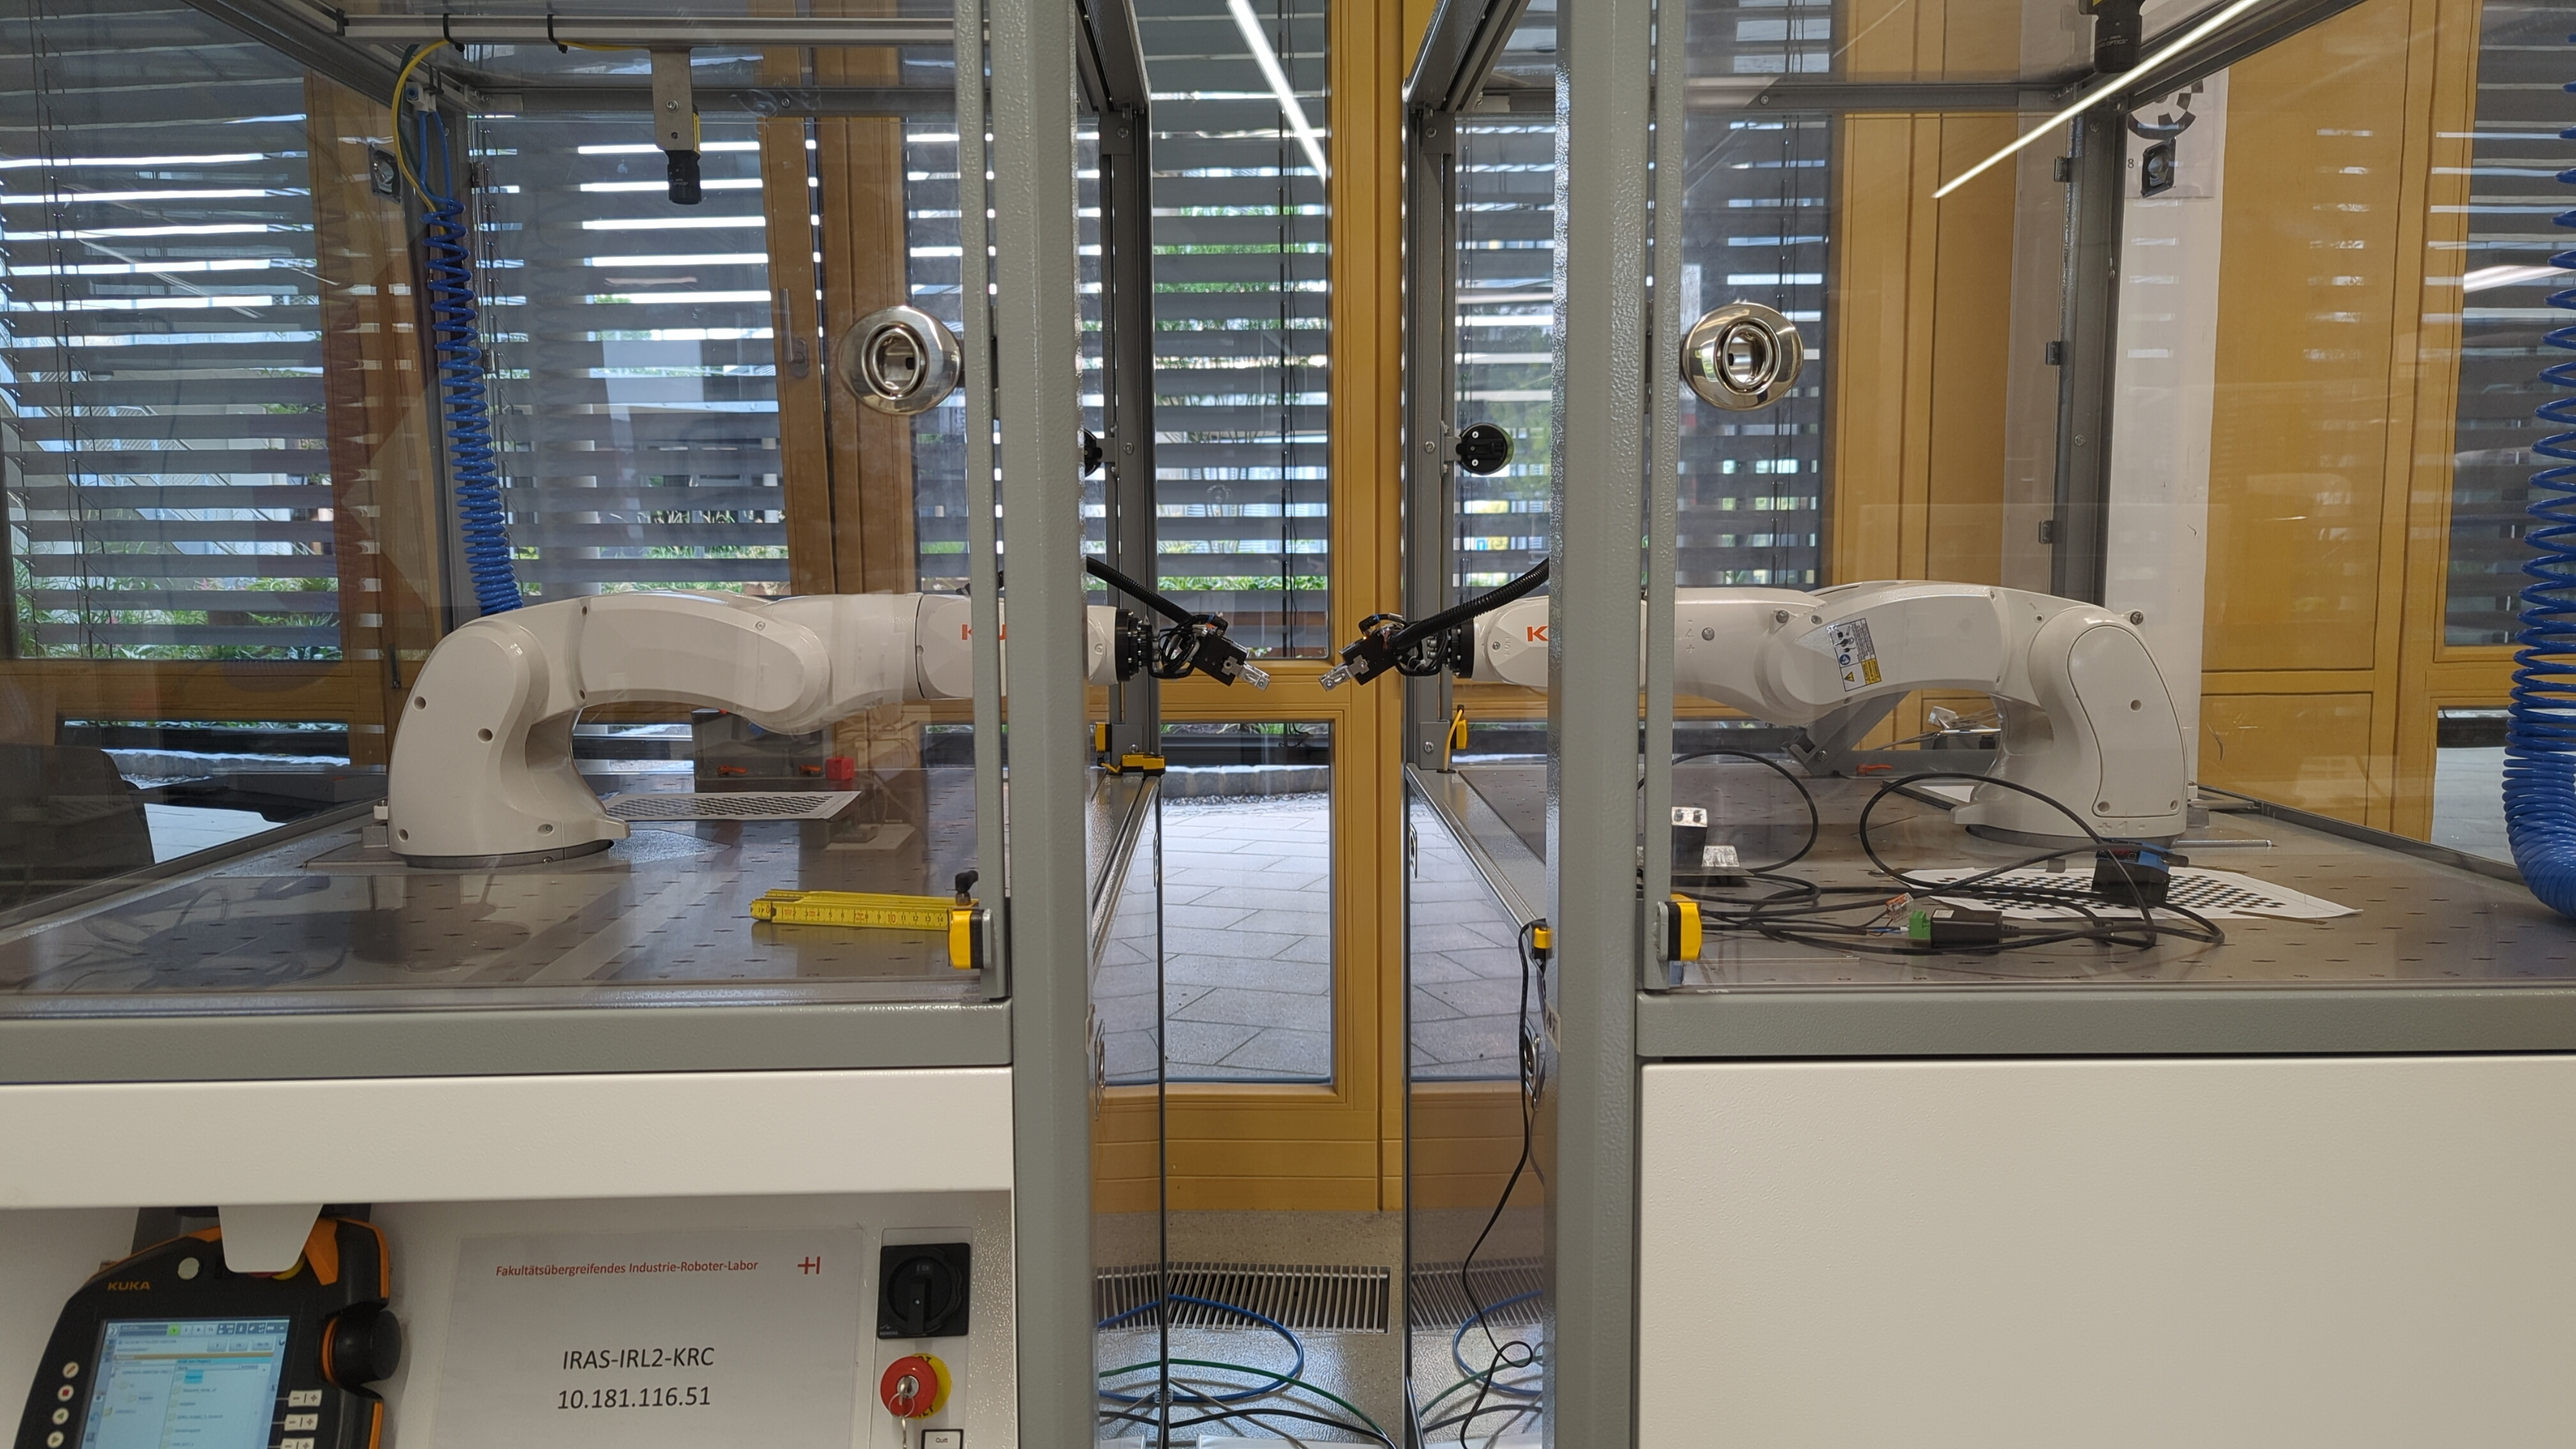
\includegraphics[width=1\textwidth]{Figures/c6/robot_placement.jpg}
	\caption{Placement of the two \textit{ready2\_educate} platforms relative to each other. The two robots are fully extended to be as close as possible to each other. }
	\label{c6_fig_robot_placement}
\end{figure}


\paragraph{Quality of Service Profiles}
There were two different \gls{qos} profiles compared, as well as three different \glspl{rmw}. An overview of the most important policy settings utilized in the \gls{qos} profiles are shown in \autoref{c6_tab_reliable_qos} and \autoref{c6_tab_sensor_qos}. For the reliable profile, the reliability was set to RELIABLE in order to guarantee to deliver the sent message. For the sensor profile, the reliability was set to BEST\_EFFORT and a queue size of five samples was used. 
\begin{table}[htbp]
    \centering
\begin{tabular}{ |c|c|c| }
\hline
\multicolumn{3}{|c|}{\gls{qos}: Reliable Profile} \\
\hline
\hline
\textbf{Policy} & \textbf{Value} & \textbf{Explanation} \\\hline
    History & KEEP\_LAST &  
        \begin{minipage}{7cm}
	       \vskip 8pt
		      We keep only the last sample.
	       \vskip 8pt
	    \end{minipage} \\\hline
    Depth & 1 &  
        \begin{minipage}{7cm}
	       \vskip 8pt
	       \vskip 8pt
	    \end{minipage} \\\hline
    Reliability & RELIABLE &  
        \begin{minipage}{7cm}
	       \vskip 8pt
		      We guarantee to deliver the sample.
	       \vskip 8pt
	    \end{minipage} \\\hline
    Durability & VOLATILE & 
        \begin{minipage}{7cm}
	       \vskip 8pt
		      Do not persist for late joining subscribers.
	       \vskip 8pt
	    \end{minipage} \\\hline
    Remaining keys & SYSTEM\_DEFAULT & 
        \begin{minipage}{7cm}
	       \vskip 8pt
		      Remaining policy parameters are set to system default.
	       \vskip 8pt
	    \end{minipage} \\\hline
\end{tabular}
    \caption{Most relevant policy parameters for the reliable profile used during evaluation. Detailed policy settings and how to configure in C++ is shown in \autoref{ca_code_qos_reliable}.}
    \label{c6_tab_reliable_qos}
\end{table}
\begin{table}[htbp]
    \centering
\begin{tabular}{ |c|c|c| }
\hline
\multicolumn{3}{|c|}{\gls{qos}: Sensor Profile} \\
\hline
\hline
\textbf{Policy} & \textbf{Value} & \textbf{Explanation} \\\hline
    History & KEEP\_LAST &  
        \begin{minipage}{7cm}
	       \vskip 8pt
		      We keep only the last 5 sample.
	       \vskip 8pt
	    \end{minipage} \\\hline
    Depth & 5 &  
        \begin{minipage}{7cm}
	       \vskip 8pt
	       \vskip 8pt
	    \end{minipage} \\\hline
    Reliability & BEST\_EFFORT &  
        \begin{minipage}{7cm}
	       \vskip 8pt
		      Only attempt to deliver samples.
	       \vskip 8pt
	    \end{minipage} \\\hline
    Durability & VOLATILE & 
        \begin{minipage}{7cm}
	       \vskip 8pt
		      Do not persist for late joining subscribers.
	       \vskip 8pt
	    \end{minipage} \\\hline
    Remaining keys & SYSTEM\_DEFAULT & 
        \begin{minipage}{7cm}
	       \vskip 8pt
		      Remaining policy parameters are set to system default.
	       \vskip 8pt
	    \end{minipage} \\\hline
\end{tabular}
    \caption{Most relevant policy parameters for the sensor profile used during evaluation. Detailed policy settings and how to configure in C++ is shown in \autoref{ca_code_qos_sensor_profile}.}
    \label{c6_tab_sensor_qos}
\end{table}


\paragraph{Evaluation Overview and Used Metrics} The combinations of which scenario, which \gls{qos} profile and which \glspl{rmw} have been combined is displayed \autoref{c6_tab_evaluation_orverview}. The different scenarios as well as their evaluation and interpretation of the evaluation are explained in detail in the following sections.\newline
In the following, $Q_1$ describes the first quartile or 25th percentile and $Q_3$ are the third quartile or 75th percentile. Outliers are values $v$ where $v<Q_1 -1.5\times IQR$ or $v>Q_3 + 1.5 \times IQR$. Score is the $R^2$ score defined as:
\begin{equation}
    R^2 = 1 - \frac{SS_{res}}{SS_{tot}}
\end{equation}
where $SS_{res}$ is the residual sum of squares and $SS_{tot}$ is the total sum of squares. The term "COEF." is short for coefficients and describes in this context the parameters for the model used by \gls{ran}. In our case, the model is a simple line in $\mathbb{R}^2$ and the coefficients are therefore the inclination of the line. And last, the term "MSE" is short for mean squared error.


\paragraph{Repositories}
The different scenarios, as well as the code and settings, used for the evaluation can be found in this  \href{https://github.com/StoglRobotics-forks/ma_demos}{repository}.\newline
The collected data, the code used for calculating the statistical measures and creation of the plots can be found in this \href{https://github.com/mamueluth/ma_evaluation}{repository}.
\begin{table}[htbp]
    \centering
\begin{tabular}{ |c|c|c|c| }
\hline
\multicolumn{4}{|c|}{Evaluation overview} \\
\hline
& eProsima Fast DDS & Eclipse Cyclone DDS & RTI Connext DDS  \\
\hline
\hline
\textbf{Scenario 1} &  &  &  \\\hline
    Sensor Profile & \checkmark & \checkmark &  \checkmark  \\\hline
    Reliable Profile& \checkmark & \checkmark &  \checkmark  \\\hline\hline
\textbf{Scenario 2} & & & \\\hline
    Sensor Profile & \checkmark & \checkmark &  \checkmark    \\\hline
    Reliable Profile &  &  &   \\\hline
\end{tabular}
    \caption{Overview of which scenario, \gls{dds} \gls{rmw} and \gls{qos} combinations were evaluated.}
    \label{c6_tab_evaluation_orverview}
\end{table}




\section{Scenario 1: Distributed Drivers}
Scenario 1 evaluates the "distributed drivers" case described in \autoref{c4_sec_distributed_drivers}. A schematic overview can be seen \autoref{c6_fig_test_scenario_1}. As shown, the scenario consists of all three computers and the two KUKA KR 3. The computers and robots were set up and connected as described in \autoref{c6_sec_setup_all}.\newline


\subsection{Experimental Setup}
As can be seen in \autoref{c6_fig_test_scenario_1}, the central controller manager was started on PC 1. The first of the two robots was controlled by PC2 and the second by PC 3. The driver for the first robot were running on PC2 and respectively the driver for the second robot on PC3. The setup on PC 2 and PC 3 was the same. They both had a sub-controller manager running and the hardware description for the robots loaded. They registered themselves at the central controller manager and exported all their \glspl{ci} and \glspl{si}. The central controller manager had a \textit{JointTrajectoryController} running which controlled both of the robots at the same time. This means the trajectory was calculated by \textit{JointTrajectoryController} on central controller manager and the commands issued to the distributed \glspl{ci}. This means that the time is implicitly synchronized, as the central controller manager calculates the command and issues them over the \gls{rmw}.\newline
The first robot was started fully extended to the front (joint\_ai = 0.0 $\forall i\in\{1,6\}$) while the second was started fully extended, but the last joint rotated 90 degree (joint\_ai = 0.0 $\forall i\in\{1,5\}$, joint\_a6 = 90). This had to do with the mounting of the distance sensor, which only looked initially pointed to the side. Then at the same time, the last joint of the first robot was rotated 90 degree counterclockwise while the last joint of the second robot was rotated 90 degree clockwise. If the target pose is reached, it was waited for approximately two seconds, then rotated back to the starting position. This process was repeated periodically. An exemplary rotation is represented in \autoref{c6_fig_schematic_gripper_mounting} through 4A and 4B. 
\begin{figure}[h]
	\centering
	\includegraphics[width=1\textwidth]{Figures/c6/test_scenario_1.pdf}
	\caption{Schematic overview of scenario 1: distributed drivers. The machines, controller manager and controller topology is shown. As can be seen, the central controller manager runs a \textit{JointTrajectoryController}, while the two distributed machines run the drivers for communication with the robots. }
	\label{c6_fig_test_scenario_1}
\end{figure}
If indeed the robots move simultaneous, then there should be no distance change during the rotation. However, as the axes of the robots around which is rotated could not be aligned perfect, we got a near and a far point. As the velocity of the rotation stays the same over the complete interval, the distance between the points should increase constant, and the measured distance points plotted versus the time look like a line. We can therefore deduce how simultaneous the robots move by measuring how good the measured distance change describes a line regarding the time. If the measured distance values form a perfect line, this indicates that the robots move simultaneous. On the other hand, a curvature or multiple curvatures of the measured distance values over the complete movement interval indicate that the robots do not move simultaneous. Further, if we repeat the process multiple times, we can compare how similar the resulting lines are and deduce the reproducibility.Jitter on the other hand is distinguishable as it has  high frequency. If the robots have a jitter during the execution of the trajectory, this results in a noisy line.\newline
For the evaluation, the distance curvature was plotted and investigated. Then the distance curvature was divided into rising and falling edges. The rising edges indicate the rotation from the starting position to the 90 degree rotated pose. The falling edge, indicating the rotation back to the start pose. The small plateaus are a result of the short stops done at reaching the goals. The plateaus were cut away, to get ascending and descending lines. This needed to be done as the precise starting point of the rotation was unknown. Then \gls{ran} was used to estimate the straight line of the rising and falling edges. It was compared how the data fits to a line. For this the minimal, maxima and mean deviation, as well as the first and third quartile of deviation from data and estimated line are plotted and compared. Note, however, that this evaluation method only holds true, as all the issued commands are generated by one source (same time for both robots) and sent over the network. Therefor, the  the difference \glspl{rmw} influences the simultaneousness by their performance or even loss of packages.
\subsection{eProsima Fast DDS}
\subsubsection{Sensor Profile}
The first test was conducted using the sensor profile and Fast DDS by eProsima as \gls{rmw}. The last joint of each robot was periodically rotated 90 degrees three times, as described previously. The distance curve over time was measured.\newline
\begin{figure}[htbp]
	\centering
	\includegraphics[width=1\textwidth]{Figures/c6/s1/s1_sensor_fast_dds.pdf}
	\caption{Distance course for scenario 1, executed with the \gls{rmw} Fast \gls{dds} by eProsima and the sensor profile. The blue curve indicates the distance change over time. The red lines are the estimated straight lines by \gls{ran} for the rising and falling edges of the distance curve.}
	\label{c6_fig_test_s1_sensor_fast_dds}
\end{figure}
The course of the distance is plotted as a blue line in \autoref{c6_fig_test_s1_sensor_fast_dds}. The distance was sampled with around 1000 samples per second (1 \si{ksps}). Before second 16, the blue line is only flat, because the execution of the trajectory has not yet begun. This is cut away. The trapezoid character of the blue line, caused by the misalignment of the axis of rotation, is clearly visible. The plateaus are caused by waiting at reaching the goal pose. The red straight line indicates the estimated model (a line in 2D space) by \gls{ran}, for each of the rising and falling edge. As can be seen in \autoref{c6_fig_test_s1_sensor_fast_dds} the measured distance values clearly follow a linear trend during the execution of the trajectory. In particular, no curvature at the start or end point of the rotations is visible. This indicates that the robots indeed move approximate simultaneous. 
At closer investigation, it can be seen that the lines have slight curvatures. This is exemplary, shown in \autoref{c6_fig_s1_sensor_fast_vs_connext} on the left side. The picture enlarges the time interval from second 16.5 to approximately second 21. For example, we can see in \autoref{c6_fig_s1_sensor_fast_vs_connext} two slight two downward bend curvatures, emphasized with the orange circles (between 17.6s and 18.3s). A longer upward bend curvature between second 19.4 and second 20.


In a next step, the deviation between the actual measured distance values and the estimated values by \gls{ran} were investigated in more detail. This was done separately for each of the rising and falling edges in \autoref{c6_fig_test_s1_sensor_fast_dds} and is displayed in \autoref{c6_fig_s1_sensor_fast_dds_box}.
\begin{figure}[htbp]
	\centering
	\includegraphics[width=1\textwidth]{Figures/c6/s1/s1_sensor_fast_dds_1_box_aio.pdf}
	\caption{Deviation of the measured values from the estimated line by \gls{ran} for the ascending and descending edges displayed in \autoref{c6_fig_test_s1_sensor_fast_dds}. The deviations are numbered in ascending order from left to right.}
	\label{c6_fig_s1_sensor_fast_dds_box}
\end{figure}
The edges are numbered in ascending order, starting with one for the farthest left edge in \autoref{c6_fig_test_s1_sensor_fast_dds}. The same applies for the descending edges. With $R^2$ scores of rounded 0.99 the estimation indicates that all the ascending values follow a linear trend very well. As can be seen, the ascending estimated lines have very similar inclinations of 0.701, 0.7, 0.696. Further, as the deviations of the ascending lines are all very centered around zero, with an interquartile range of about 4 \si{\micro\meter} and a maximal deviation of roughly 8 \si{\micro\meter}. With 24 the most outliers, are measured for the ascending second ascending edge. The values for the descending edges are similarly close together as it is for the ascending deviations, the case. This reinforces the claim of the robots moving in a quite simultaneous manner. Moreover, it shows that the movement has a high repeatability.
\subsubsection{Reliable Profile}
For the reliable profile, the same procedure as for the sensor profile was conducted. However, the experiments were conducted at a later time and the first thing to note is that both the near and far point shifted by around +500 \si{\micro\meter}.
It is not clear why this happened. One explanation could be that the sensor or plate moved, as they are not bolted down but rather gripped. This should not compromise the results as the estimated line and therefore the deviation is calculated relative to the values.\newline 
The results for the first three rotations are shown in \autoref{c6_fig_s1_reliable_fast_box_aio}. Again, no curvature at the start or end point of the rotations is visible. During the executions, the linear trend is clearly visible. The lines described by the rising and falling edges of the distance curve are estimated with \gls{ran}. Then the deviation for each ascending and descending edge from the estimated model is calculated. With all \gls{r2} scores around 0.99, the result again clearly describe a line. The inclinations are with around 0.69 about the same as for the sensor profile case. The minimal and maximal deviation are slightly higher, as for the sensor profile case. 
\begin{figure}[htbp]
	\centering
	\includegraphics[width=1\textwidth]{Figures/c6/s1/s1_reliable_fast_dds_3_box_aio.pdf}
	\caption{Fast DDS as \gls{rmw} and the reliable profile are used for execution of scenario 1. Deviations of the measured distance values and estimated values for the ascending and descending edges of the first three rotations.}
	\label{c6_fig_s1_reliable_fast_box_aio}
\end{figure}
The \gls{iqr} is slightly higher as for the sensor profile case. The \gls{mse} is slightly higher as well. In comparison to the sensor profile there are over all more outliers and the maximum number of outliers is with 79 in comparison to 24 in the sensor profile execution about three times as high.\newline
In \autoref{c6_fig_s1_fast_reliable_vs_sensor} the first ascending edges are plotted. On the left side, the distance curve for the reliable profile, as well as the estimated line, is displayed. On the right side, the distance curve and estimated line for the sensor profile are shown. The blue lines are the distance curves, the red lines are the estimated lines by \gls{ran}. As indicated by the calculated metrics for the deviations in \autoref{c6_fig_s1_reliable_fast_box_aio} the lines look very similar. For the most parts, as for example indicated with the black circles, both lines clearly follow a linear trend and have minor deviations. The orange circles indicate where the distance values experience the greatest curvature. As can be seen, the curvature is slightly greater when the reliable profile is used. This holds true for nearly all the executions.


Altogether, the robots move nearly simultaneous, with slight curvatures in the distance curve. This is holds true no matter if the reliable or sensor profile is used, indicating that neither if the reliable nor if the sensor profile can guarantee a complete simultaneous execution. The sensor profile seems to perform slightly better, but no significant differences are found. With both the reliable and sensor profile no jitter is observed. Overall, the simultaneousness and repeatability of the robot motion in both cases is good.
\begin{figure}[hhtpb]
	\centering
	\includegraphics[width=1\textwidth]{Figures/c6/s1/s1_fast_dds_reliable_vs_sensor.png}
	\caption{Comparison of the reliable and sensor profile when using Fast \gls{dds} by eProsima. Reliable profile displayed on the left, sensor profile on the right. Distance values for the first rotation in blue. Estimated line for the values by \gls{ran} in red. Orange show the greatest curvature in the line. The black circle shows that lines are very similar for the most part.}
	\label{c6_fig_s1_fast_reliable_vs_sensor}
\end{figure}

\subsection{Eclipse Cyclone DDS}\todo{Kein über oder untersteuern am start}
\subsubsection{Sensor Profile}
Next, Cyclone \gls{dds} was used as \gls{rmw}. The sensor profile was used. In \autoref{c6_fig_s1_sensor_cyclone} the distance curve for the three rotations is shown. The sample rate was around 1 ksps. As can be seen, during the rotation the distance curve follows a clear linear trend. This is backed up by \autoref{c6_fig_s1_sensor_cyclone_box_aio}. In \autoref{c6_fig_s1_sensor_cyclone_box_aio} it is shown, that the \gls{r2} score for each of the ascending and descending edges is 0.999, which underlines this. All the minimal deviations are centered around -0.066, and the maximal deviations around 0.069. With the interquartile ranges around 0.039 indicating that the measured distance values are very close to the estimated trend by \gls{ran}. At closer investigation in can again seen, that for example in the upper third of the execution there is a slight curvature in the line, meaning the robots move not perfectly simultaneous. However, with the measured absolute maximal deviation of 0.073 \si{\milli\meter}, the robots are moving quasi simultaneous.\newline
With inclinations of 0.702 for each of the ascending edges and inclinations of around -0.0704 for all the descending edges, the executed motion seems to be repeated reliable. This is also underlined by the fact that all the calculated metrics are lying close together. Further, no jitter is measurable. 
\begin{figure}[htbp]
	\centering
	\includegraphics[width=1\textwidth]{Figures/c6/s1/s1_sensor_cyclon_dds.pdf}
	\caption{Cyclone DDS as \gls{rmw} and the sensor profile are used for execution of scenario 1. Deviations of the measured distance values and estimated values for the ascending and descending edges of the first three rotations.}
	\label{c6_fig_s1_sensor_cyclone}
\end{figure}
\begin{figure}[htbp]
	\centering
	\includegraphics[width=1\textwidth]{Figures/c6/s1/s1_sensor_cyclone_dds_1_box_aio.pdf}
	\caption{Deviation of the measured values from the estimated line by \gls{ran} for the ascending and descending edges displayed in \autoref{c6_fig_s1_sensor_cyclone}. The deviations are numbered in ascending order from left to right.}
	\label{c6_fig_s1_sensor_cyclone_box_aio}
\end{figure}
\subsubsection{Reliable Profile}
For the execution with the reliable profile, the average values for three rotations for the rising and falling edges can be found in \autoref{c6_tab_result_overview}. The values in the table are the averages of the three rising and falling edges. As can be seen, the values for the reliable profile are close to the values of the sensor profile. The sensor profile is except for the outlier count of the rising edges at least as good as the reliable profile. This indicates, that the sensor profile's performances is slightly better than the performance of the reliable profile.


In summary, with Cyclone \gls{dds} by Eclipse, the robots move nearly simultaneous. There are slight curvatures in the distance curve, while the trajectory is executed, indicating that the robots do not move complete in sync. However, the deviations are in the sub micro meter scale and over all the movement is nearly simultaneous. The reliable profile seems to perform slightly worse than the sensor profile, probably due to the overhead of granting that samples are received. Neither with the reliable nor with the sensor profile, the robots experience jitter.
\subsection{RTI Connext DDS}\todo{Kein über oder untersteuern am start}
\subsubsection{Sensor Profile}The distance curve for the executed rotations when Connext DDS by RTI is used as \gls{rmw} is shown in \autoref{c6_fig_s1_sensor_connext}. As can be seen, the line is very noise compared to Fast \gls{dds} and Cyclone \gls{dds}.
\begin{figure}[htbp]
	\centering
	\includegraphics[width=1\textwidth]{Figures/c6/s1/s1_sensor_connext_dds.pdf}
	\caption{Connext DDS as \gls{rmw} and the sensor profile are used for execution of scenario 1. Deviations of the measured distance values and estimated values for the ascending and descending edges of the first three rotations. The robots experienced a lot of jitter.}
	\label{c6_fig_s1_sensor_connext}
\end{figure}
This indicates that the robots experienced high jitter during the execution. While the tests were conducted, the jitter was clearly visibly with the bare eye. The distance curve during the movement still clearly follows a linear trend, but the values have a higher variance, which is expected due to the jitter. As indicated by the distance curve, the robots still move more or less simultaneous, as no big curvature is visible.\newline
In \autoref{c6_fig_s1_connext_box_aio} the results for the metrics for the deviations from the estimated trend by \gls{ran} are shown. The overall results have a much higher variance in between the repeated motion. Compared to the execution with the sensor profile by Fast \gls{dds} and Cyclone \gls{dds}, the minimal and maximal deviations are with an absolute maximal deviation of 0.122 are significant higher. The same applies for the outlier count, where Connext DDS with an average of 110 outliers is about 20 times higher than the count of Fast DDS and about 84 times higher than the count for Cyclone DDS. Further, the \gls{iqr} of Connext DDS is wider than those of Fast DDS and Cyclone DDS, which is due to the high jitter. The jitter also leads to a significant increased \gls{mse}
\begin{figure}[htbp]
	\centering
	\includegraphics[width=1\textwidth]{Figures/c6/s1/s1_sensor_connext_dds_1_box_aio.pdf}
	\caption{Deviation of the measured values from the estimated line by \gls{ran} for the ascending and descending edges displayed in \autoref{c6_fig_s1_sensor_connext}. The deviations are numbered in ascending order from left to right.}
	\label{c6_fig_s1_connext_box_aio}
\end{figure}
\subsubsection{Reliable Profile}\todo{Maybe bit more}
When using the reliable profile for Connext DDS the jitter increases further. This is visible in the higher \gls{iqr}, greater standard deviation and greater absolute deviation in \autoref{c6_tab_evaluation_orverview}. This is consistent with the result before, as the reliable profile always performs slightly worse than the sensor profile.

It can be concluded that with Connext DDS the robots still move in a synchronous manner. No big curvatures are visible during the executed motions. However, the robots experience significant jitter during the execution. As with Fast DDS and Cyclone DDS the sensor profile performs better than the reliable profile.
\section{Summary}
In \autoref{c6_tab_evaluation_orverview} the average for the execution of three rotations is show. Compared are Fast \gls{dds} by eProsima, Cyclone \gls{dds} by Eclipse and Connext \gls{dds} by RTI, as well as the reliable and sensor profile. The results are divided in the average results for the ascending edge in the upper part of the table and the average results of the descending edge in the lower part. The blue highlighted values indicate the best value for each row, while the red highlighting indicates the worst value.
\begin{table}[htbp]
\begin{tabular}{|l|ll|ll|ll|}
\toprule
\multicolumn{7}{|c|}{Average Result of Three Ascending and Three Descending Lines} \\
\toprule
 RMW & Fast & Fast  & Cyclone & Cyclone & Connext & Connext \\
\midrule
Profile & sensor & reliable & sensor & reliable & sensor & reliable \\
\midrule
Line & asc. & asc. & asc. & asc. & asc. & asc. \\
Min & -0.076 & -0.087 & \textcolor{blue}{\textbf{-0.065}} & -0.067 & -0.097 & \textcolor{red}{\textbf{-0.123}} \\
Max & 0.078 & 0.087 & \textcolor{blue}{\textbf{0.072}} & \textcolor{blue}{\textbf{0.072}} & 0.097 & \textcolor{red}{\textbf{0.119}} \\
Mean & -0.003 & \textcolor{red}{\textbf{-0.005}} & -0.004 & -0.004 & \textcolor{blue}{\textbf{-0.001}} & 0.002 \\
std. deviation & 0.029 & 0.035 & \textcolor{blue}{\textbf{0.026}} & 0.029 & 0.040 & \textcolor{red}{\textbf{0.048}} \\
\gls{q1} & -0.021 & -0.021 & -0.020 & -0.021 & -0.025 & -0.030 \\
\gls{q3} & 0.020 & 0.022 & 0.018 & 0.019 & 0.024 & 0.032 \\
\gls{iqr} & 0.042 & 0.043 & \textcolor{blue}{\textbf{0.038}} & 0.04 & 0.049 & \textcolor{red}{\textbf{0.063}} \\
Outliers & 8.000 & \textcolor{red}{\textbf{90.667}} & 2.667 & \textcolor{blue}{\textbf{0.000}} & \textcolor{red}{\textbf{90.667}} & 68.667 \\
\gls{r2} score & \textcolor{blue}{\textbf{0.999}} & 0.998 & \textcolor{blue}{\textbf{0.999}} & \textcolor{blue}{\textbf{0.999}} & 0.997 & \textcolor{red}{\textbf{0.996}} \\
Coef. & 0.699 & 0.687 & 0.702 & 0.701 & 0.684 & 0.697 \\
\gls{mse} [1e-3] & 0.829 & 1.193 & \textcolor{blue}{\textbf{0.680}} & 0.851 & 1.655 & \textcolor{red}{\textbf{2.351}} \\
\midrule
Line & desc. & desc. & desc. & desc. & desc. & desc. \\
Min & \textcolor{blue}{\textbf{-0.066}} & -0.089 & -0.067 & -0.067 & -0.094 & \textcolor{red}{\textbf{-0.107}} \\
Max & 0.069 & 0.086 & \textcolor{blue}{\textbf{0.067}} & 0.073 & 0.097 & \textcolor{red}{\textbf{0.108}} \\
Mean & -0.004 & \textcolor{red}{\textbf{-0.006}} & -0.002 & -0.004 & \textcolor{blue}{\textbf{0.000}} & 0.002 \\
std. deviation & \textcolor{blue}{\textbf{0.025}} & 0.034 & 0.027 & 0.029 & 0.043 & \textcolor{red}{\textbf{0.042}} \\
\gls{q1} & -0.018 & -0.023 & -0.019 & -0.021 & -0.022 & -0.028 \\
\gls{q3} & 0.017 & 0.022 & 0.018 & 0.018 & 0.026 & 0.027 \\
\gls{iqr} & \textcolor{blue}{\textbf{0.035}} & 0.045 & 0.037 & 0.039 & 0.048 & \textcolor{red}{\textbf{0.055}} \\
Outliers & 2.667 & 40.000 & \textcolor{blue}{\textbf{0.000}} & 0.333 & \textcolor{red}{\textbf{129.333}} & 53.667 \\
\gls{r2}score & \textcolor{blue}{\textbf{0.999}} & 0.998 & \textcolor{blue}{\textbf{0.999}} & \textcolor{blue}{\textbf{0.999}} & \textcolor{red}{\textbf{0.997}} & \textcolor{red}{\textbf{0.997}} \\
Coef. & -0.707 & -0.689 & -0.704 & -0.702 & -0.698 & -0.694 \\
\gls{mse} [1e-3] & \textcolor{blue}{\textbf{0.604}} & 1.151 & 0.712 & 0.827 & \textcolor{red}{\textbf{1.949}} & 1.757 \\
\bottomrule
\end{tabular}
    \centering
    \caption{Comparison of the average result for the three ascending and descending lines. Compared are Fast DDS, Cyclone DDS and Connext DDS as well as the sensor and reliable profile. Best result is shown in blue, worst in red.}
    \label{c6_tab_result_overview}
\end{table}
The first thing to note is, that with the sensor profile deviations are always smaller than with the reliable profile. This is probably caused by the overhead generated by the fact that the reliable profile guarantees reliable transmission of the messages. On the other hand, as the network was not utilized by any other applications and only the traffic generated by the conducted test was routed over the network, there probably wasn't a high loss of messages by the sensor profile.\newline
Further, Cyclone DDS has the slightly smaller deviations than Fast DDS. They are however almost negligible. Connext DDS hast the highest deviations caused by the jitter. The jitter is the greatest observable difference between the different \glspl{rmw}. In\autoref{c6_fig_s1_sensor_fast_vs_connext} the measured distance values for the first rising edge for Fast DDS and Connext DDS are displayed. The values for Fast DDS are on the left, those for Connext DDS are on the right.
\begin{figure}[htbp]
	\centering
	\includegraphics[width=1\textwidth]{Figures/c6/s1/s1_sensor_fast_vs_connext.png}
	\caption{Comparison of Fast \gls{dds} by eProsima on the left side and Connext \gls{dds} by RTI on the right side. Both depict the first rising edge of the distance curve for scenario 1 with the sensor profile. Orange circles show curvatures in the line, indicating that the robots did not move perfectly simultaneous. The black circle indicates exemplary a region where the robot experienced high jitter. }
	\label{c6_fig_s1_sensor_fast_vs_connext}
\end{figure}
The jitter is clearly visible, this is highlighted with the black circle. As can be seen, the jitter is present during the whole execution, even after the rotation stopped. Additional, in the orange circles, some areas are highlighted where a curvature is visible.

In summary, that the usage of a sensor profile yields better results than the usage of a reliable profile. Cyclone DDS performs slightly better than Fast DDS, the difference however seems negligible. With both Cyclone DDS and Fast DDS the robots move almost synchronous with only slight curvatures visible in the measured distance values. The executed trajectory hardly shows any deviations between several executions. Neither Cyclone DDS nor Fast DDS experience any jitter. With Connext DDS significant jitter is experienced.


\section{Scenario 2: Distributed Chained Control}
Scenario 2 evaluates the "distributed chained control" case described in \autoref{c4_sec_distributed_controller_chaining}. A schematic overview can be seen in \autoref{c6_fig_test_scenario_2}. As shown, the scenario consists of all three computers and the two KUKA KR3 R540. The computers and robots were connected and set up as described in \autoref{c6_sec_description}.

\subsection{Experimental Setup}
As can be seen in \autoref{c6_fig_test_scenario_2} the central controller manager was started on PC1. The central controller manager had a \textit{FowardCommandController}running. The sub-controller managers were started on PC2 and PC3. The drivers for controlling the first robot were run on PC2 and the driver for controlling the second robot were run on PC3. In addition to the driver on PC2 and PC3, on each of the sub-controller managers had a \textit{JointTrajectoryController} running. The \textit{ForwardCommandController} on the central controller manager. This means that the \textit{JointTrajectoryControllers} of the sub-controller managers claim the \glspl{ci} locally, create \glspl{ri} and register them at the central controller manager. With this setup, \textit{ForwardCommandController} creates a trajectory message. The trajectory message is then sent to the \textit{JointTrajectoryControllers} input via the exported reference interfaces. This means that in comparison to scenario 1 where the central controller manager's \textit{JointTrajectoryController} \textit{JointTrajectoryControllers} were then chained to the calculated the issued commands in order to execute the trajectory, this was now separate for each robot by the \textit{JointTrajectoryControllers} of the sub-controller managers. This greatly reduces the traffic sent over the \gls{rmw}, as only one trajectory message every few second needs to be sent instead of the calculated values for the \glspl{ci}. On the other hand, as the time of the computers is not synchronized a unary start of the execution of the trajectory can not be expected. As a result, the influence of the used \gls{rmw} restricted to the initial "JointTrajectory message" sent via the \gls{ri}. After the message has been sent, the commands are calculated per sub-controller manager and the robot is controller via \gls{rsi}. \newline
As in scenario 1 the first robot was started fully extended to the front (joint\_ai = 0.0 $\forall i\in\{1,6\}$) while the second was started fully extended, but the last joint rotated 90 degree (joint\_ai = 0.0 $\forall i\in\{1,5\}$, joint\_a6 = 90). Then at the same time, the last joint of the first robot was rotated 90 degree counterclockwise while the last joint of the second robot was rotated 90 degree clockwise. If the target pose is reached, it was waited for a short time, then rotated back to the starting position. This process was repeated periodically. An exemplary rotation is represented in 
\begin{figure}[htbp]
	\centering
	\includegraphics[width=1\textwidth]{Figures/c6/test_scenario_2.pdf}
	\caption{Schematic overview of scenario 2: distributed chained controllers. The machines, controller manager and controller topology is shown. As can be seen, the central controller manager runs a \textit{ForwardCommandController}, while the two distributed machines run a \textit{JointTrajectoryController} and the drivers for communication with the robots. The output of the \textit{ForwardCommandController} ins chained to each of the inputs of the \textit{JointTrajectoryController}.}
	\label{c6_fig_test_scenario_2}
\end{figure}
\autoref{c6_fig_schematic_gripper_mounting} through 4A and 4B.\newline
\begin{figure}[htbp]
	\centering
	\includegraphics[width=1\textwidth]{Figures/c6/s2/s2_fast_vs_connext.png}
	\caption{Distance course for one rotation. The measured distance values are in blue, the estimated trend of the values in red. On the left is Fast DDS as \gls{rmw} on the right Connext DDS. The orange circle indicates clear deviations at the start and end of the rotation, meaning that the robots did not start to move simultaneous.}
	\label{c6_fig_s2_fast_vs_connext}
\end{figure}
In \autoref{c6_fig_s2_fast_vs_connext} en example rotation is shown. On the left side for Fast DDS and on the right site for Connext DDS. The measured distance values are plotted in blue, and the estimated line by \gls{ran} is displayed in red. The orange circles highlight clearly visible deviations immediately after the start and near the end of the rotations, as the robots do not start in sync. During the rotation, the line is nearly perfectly linear.The effect is in particular visible for Connext DDS. At the star of the rotation (at about 23.25s) we get a very steep curvature as only the first robot starts moving. Then the second robot starts moving as well ant the distance curve is linear with newly no deviations visible. Then as the first robot reaches the goal pose and waits, we can again see a big curvature, indicating the closing in of the second robot on the goal pose.\newline
This is expected, as the created motion by the \textit{JointTrajectoryControllers} of the sub-controller manager output a constant velocity. Meaning the robots may not start simultaneous, but once they start moving the move bot at a constant speed. As already mentioned before, the \gls{rmw} does not influence this, as the commands are no longer set via \gls{dds} and then via the driver over the \gls{rsi} to the robot controller, but instead are issued locally to the \gls{ci} and then via the driver and \gls{rsi} to the robot controller. This is a distinct difference to scenario 1 as the time of the execution is not synchronized. As a result, the curvatures at the beginning and end of the executions vary greatly. The trend of Connext DDS performing a worse than its competitors seem to continue, as the curvatures with Connext DDS  are greater than those seen with Fast DDS or Connext DDS. This is probably due to the fact, that the "Trajectory messages" sent over the \glspl{ri} arrive with a greater time lag than it is the case with Fast DDS or Connext DDS. However, the collected data consist only of around 30 rotations for each \gls{rmw}, further investigation should be done.

In summary, the concept of distributed chained control works. The arrival of the "Trajectory messages" influences the start time of each of the robots motions. The results indicate, that in order to guarantee a simultaneous start of the further synchronization is needed. 

\section*{Side Note}
The concept has also been tested with a KUKA KR 5 and a KUKA KR 16-2. One notable difference is that the industrial controllers for those two robots have different cycle time. For communication with the KUKA KR 5 over the \gls{rsi} the controller expects a period of 4 \si{\milli\second}, while the controller of the KUKA KR 16-2 expects a cycle time of 12 \si{\milli\second}. The robots seemed to move in sync, however a detailed analysis could not be conducted. The robots are about 5m away from each other, with the reach of the distance sensor an evaluation was not feasible. 
% \begin{itemize}
%     \item \todoin{should probably test with different network workloads}
%     \item \todoin{Different Publishing types}
%         \begin{enumerate}
%             \item Node topology
%             \item Publish trigger
%             \item Publish type 
%         \end{enumerate}
%     \item \todoin{What about Zenoh?}
% \end{itemize}